\documentclass{article}

\newcommand*{\plogo}{\fbox{$\mathcal{PL}$}}

\usepackage{indentfirst}
\usepackage{anysize}
\usepackage{graphicx}
\usepackage{subfigure}
\usepackage{array}
\usepackage{makecell}
\usepackage{CJK}

\usepackage{fancyhdr}
\pagestyle{fancy}
%\usepackage[colorlinks=true,linkcolor=black,citecolor=magenta,urlcolor=red]{hyperref}
%\usepackage[all]{hypcap}

\linespread{1.2}


\marginsize{3cm}{3cm}{1cm}{1cm}
\setlength{\parindent}{2em}

\newcolumntype{L}[1]{>{\vspace{0.5em}\begin{minipage}{#1}\raggedright\let\newline\\
\arraybackslash\hspace{0pt}}m{#1}<{\end{minipage}\vspace{0.5em}}}
\newcolumntype{R}[1]{>{\vspace{0.5em}\begin{minipage}{#1}\raggedleft\let\newline\\
\arraybackslash\hspace{0pt}}m{#1}<{\end{minipage}\vspace{0.5em}}}
\newcolumntype{C}[1]{>{\vspace{0.5em}\begin{minipage}{#1}\centering\let\newline\\
\arraybackslash\hspace{0pt}}m{#1}<{\end{minipage}\vspace{0.5em}}}

%使得图片显示对应章节
\renewcommand\thefigure{\thesection.\arabic{figure}}
\makeatletter
\@addtoreset{figure}{section}
\makeatother


\begin{document}
\begin{CJK}{UTF8}{gbsn}
%页眉、页脚设置
\lhead{
	\setlength{\unitlength}{1mm}
        \begin{picture}(0,0)
        \put(0,0){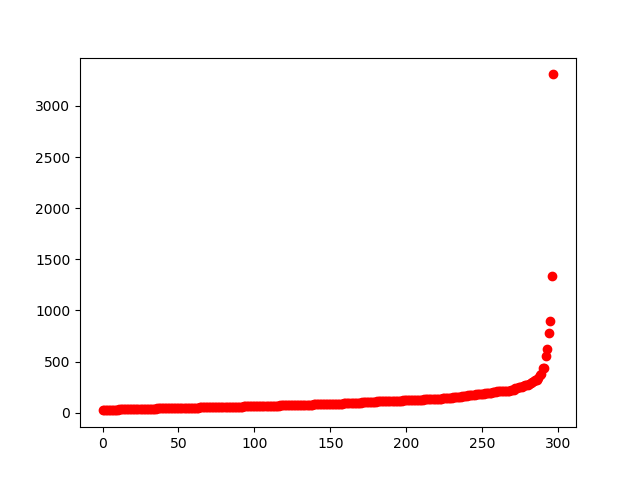
\includegraphics[width=0.7cm]{1.jpg}}
        \end{picture}
}
\chead{}
\rhead{\bfseries DAM-2018}
\lfoot{\itshape Tongji University}
\cfoot{\thepage}
\rfoot{\itshape School of Software Engineering}
\renewcommand{\headrulewidth}{0.4pt}
\renewcommand{\footrulewidth}{0.4pt}

\newcommand*{\titleGP}{\begingroup % Create the command for including the title page in the document
\centering % Center all text
\vspace*{\baselineskip} % White space at the top of the page

\rule{\textwidth}{1.6pt}\vspace*{-\baselineskip}\vspace*{2pt} % Thick horizontal line
\rule{\textwidth}{0.4pt}\\[\baselineskip] % Thin horizontal line

{\LARGE 超市数据的频繁项集挖掘 -- b问分析文档
 \\ \vspace{2em} \begin{large} 数据分析与数据挖掘 \end{large}}\\[0.2\baselineskip] % Title

\rule{\textwidth}{0.4pt}\vspace*{-\baselineskip}\vspace{3.2pt} % Thin horizontal line
\rule{\textwidth}{1.6pt}\\[\baselineskip] % Thick horizontal line

\scshape % Small caps
%周一  饶卫雄老师 \\[\baselineskip] % Tagline(s) or further description
DAM COURSE, SPRING 2018\par % Location and year

\vspace*{2\baselineskip} % Whitespace between location/year and editors

 BY \\[\baselineskip]
{\Large 1552674 李\quad 源  \par} % Editor list


\vspace{23em}
\begin{figure}[!h]
\begin{center}
  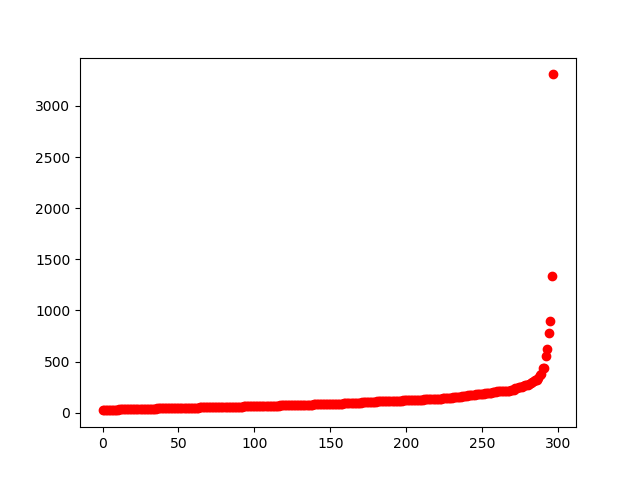
\includegraphics[width = 0.2\textwidth]{1.jpg}	
\end{center}
\end{figure}
\vfill

{\itshape Tongji University \\ School of Software Engineering \par} % Editor affiliation
\endgroup}

\titleGP % This command includes the title page
\thispagestyle{empty}
\clearpage


\section{trade\_new.csv文件数据代码运行结果}
\subsection{数据预处理耗时}

针对bi问的数据预处理时间如下:
\begin{figure}[!h]
\begin{center}
  \includegraphics[width = 0.9\textwidth]{bi.png}	
\end{center}
\end{figure}

针对bii问的数据预处理时间如下:
\begin{figure}[!h]
\begin{center}
  \includegraphics[width = 0.9\textwidth]{bii.png}	
\end{center}
\end{figure}

\subsection{bi问针对三个字段的频繁集求取情况}
\subsubsection{频繁集个数}
针对pluno、dptno、bndno字段,在2、4、8、16、32、64分别作为最小支持度时,频繁集个数:

\begin{figure}[!h]
\begin{center}
  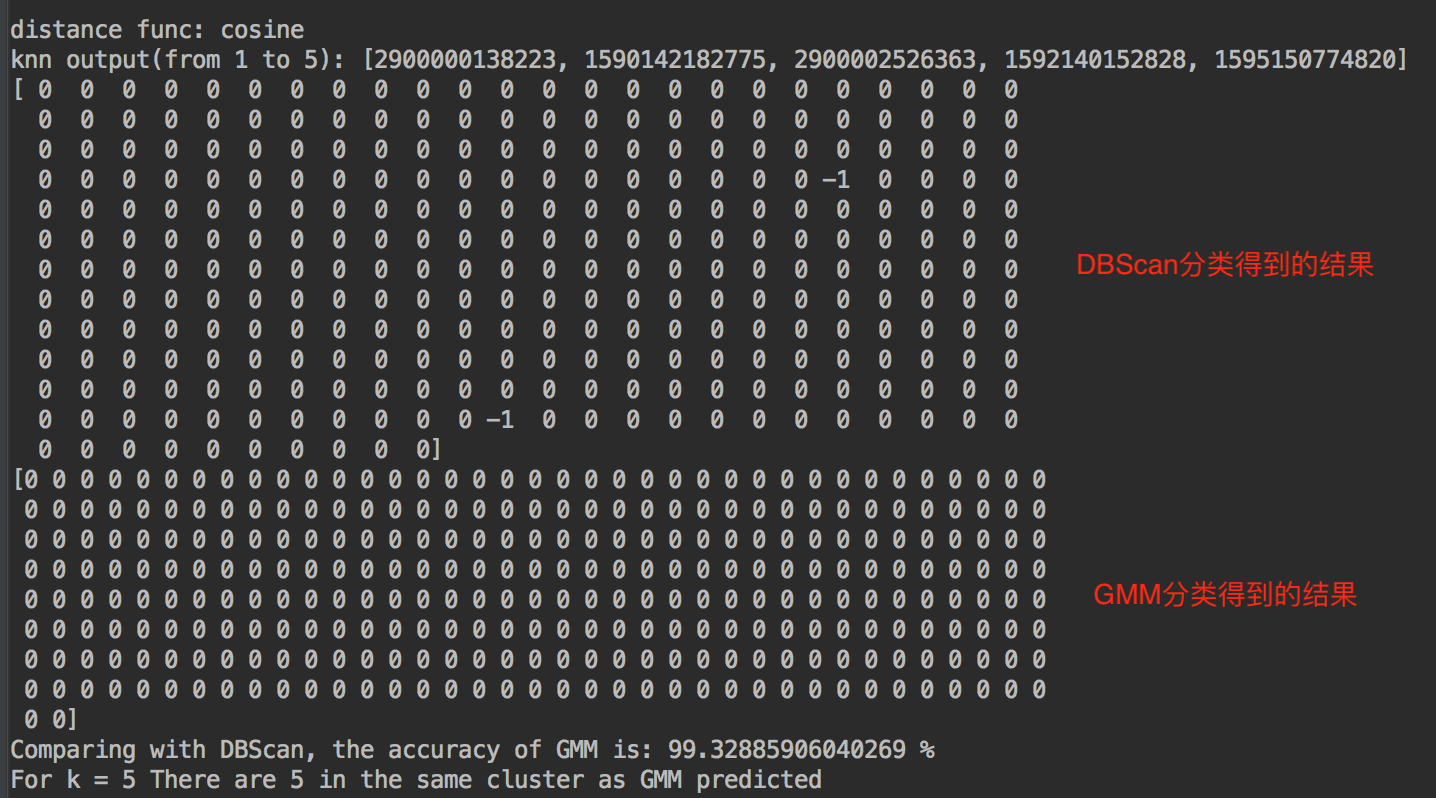
\includegraphics[width = 0.9\textwidth]{2.png}	
\end{center}
\end{figure}

\clearpage
\subsubsection{运行时间}
针对pluno、dptno、bndno字段,在2、4、8、16、32、64分别作为最小支持度时,运行时间:
\begin{figure}[!h]
\begin{center}
  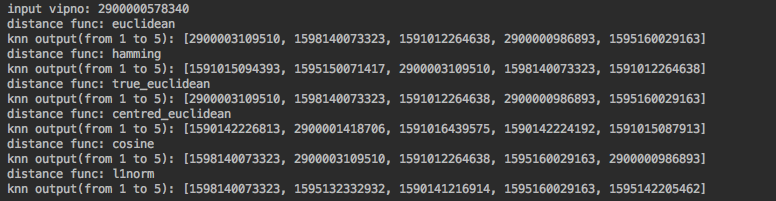
\includegraphics[width = 0.9\textwidth]{3.png}	
\end{center}
\end{figure}

\subsubsection{具体输出}
针对pluno、dptno、bndno字段,在16作为最小支持度时,使用SPMF包获得的输出结果:

pluno字段:
\begin{figure}[!h]
\begin{center}
  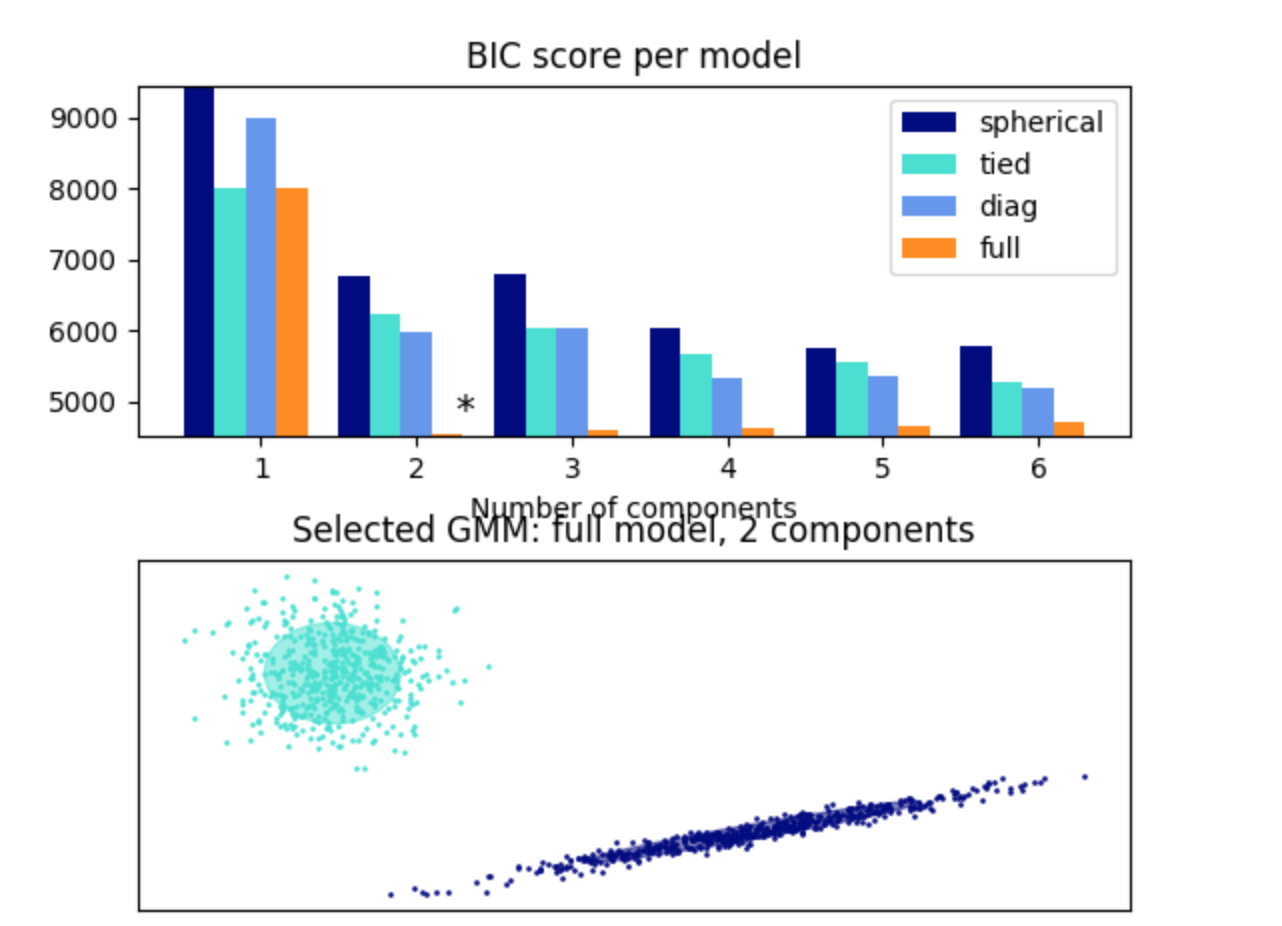
\includegraphics[width = 0.8\textwidth]{4.png}	
\end{center}
\end{figure}

dptno字段:
\begin{figure}[!h]
\begin{center}
  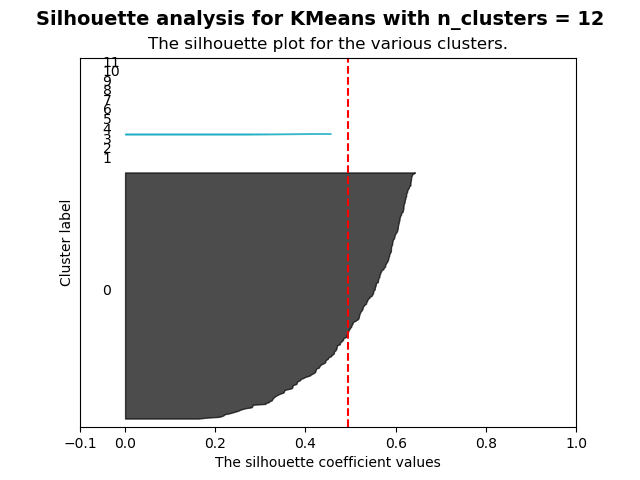
\includegraphics[width = 0.8\textwidth]{5.png}	
\end{center}
\end{figure}

bndno字段:
\begin{figure}[!h]
\begin{center}
  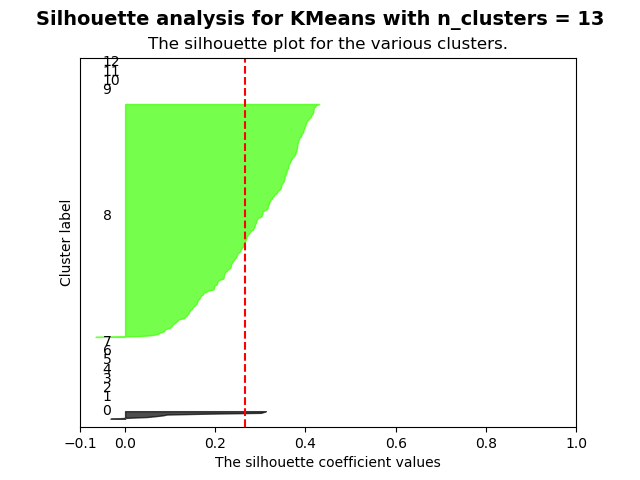
\includegraphics[width = 0.8\textwidth]{6.png}	
\end{center}
\end{figure}


\subsection{bii问针对三个字段的频繁集求取情况}
\subsubsection{频繁集个数}
针对pluno、dptno、bndno字段,在2、4、6、8、10分别作为最小支持度时,频繁集个数:

\clearpage
\begin{figure}[!h]
\begin{center}
  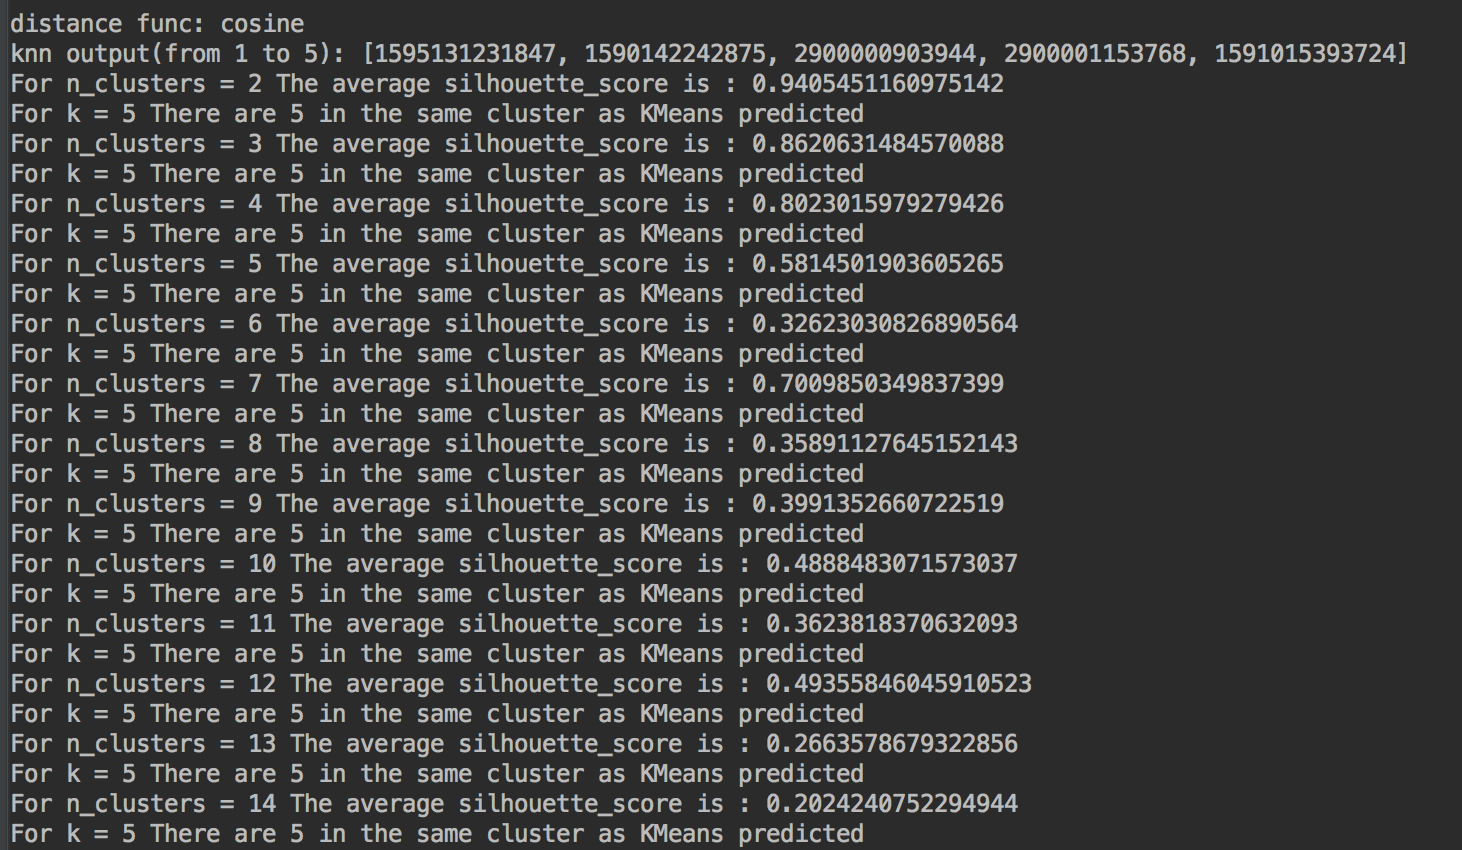
\includegraphics[width = 0.9\textwidth]{7.png}	
\end{center}
\end{figure}

\subsubsection{运行时间}
针对pluno、dptno、bndno字段,在2、4、6、8、10分别作为最小支持度时,运行时间:
\begin{figure}[!h]
\begin{center}
  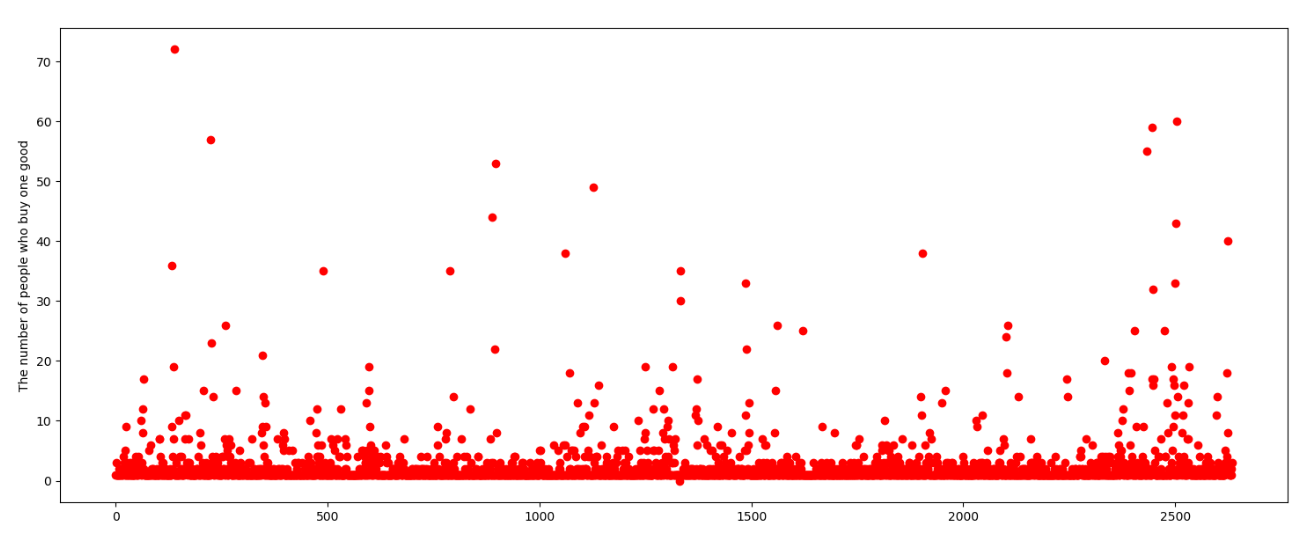
\includegraphics[width = 0.9\textwidth]{8.png}	
\end{center}
\end{figure}

我在这里选择的是PrefixSpan算法。

总的来说,除了对应dptno字段在最小支持度为2的时候,所耗时间较长之外,其他的运行时间都比较短,同时与a问的FP-growth算法相比,基本上差异不大,可见两者的性能差异不大。而对于频繁项集的结果,我将会在分析讨论中做一个详细说明。

\section{trade.csv文件数据代码运行结果}

针对bi问的数据预处理时间如下:
\clearpage
\begin{figure}[!h]
\begin{center}
  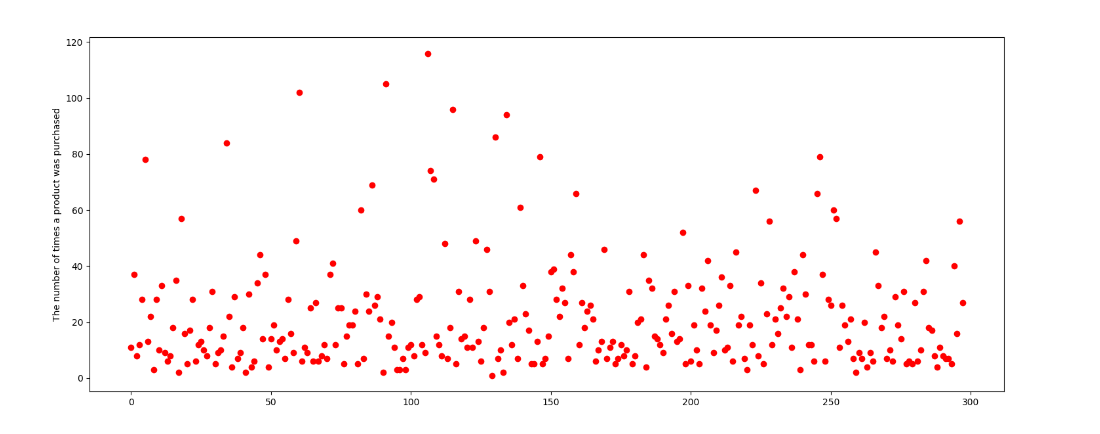
\includegraphics[width = 0.7\textwidth]{9.png}	
\end{center}
\end{figure}

针对bii问的数据预处理时间如下:

\begin{figure}[!h]
\begin{center}
  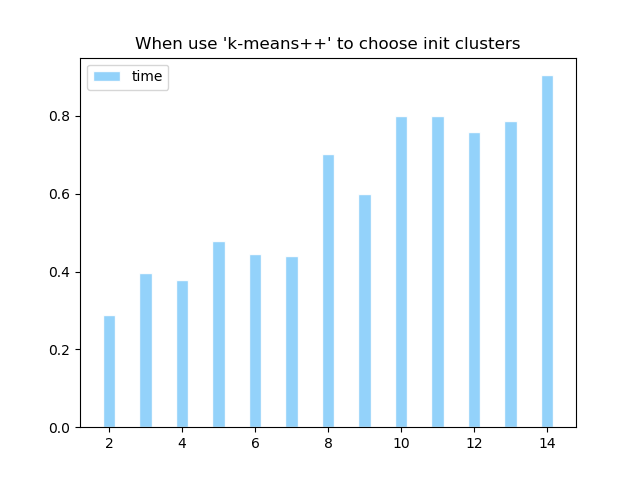
\includegraphics[width = 0.7\textwidth]{10.png}	
\end{center}
\end{figure}


\subsection{bi问针对三个字段的频繁集求取情况}
\subsubsection{频繁集个数}
针对pluno、dptno、bndno字段,在2、4、8、16、32、64分别作为最小支持度时,频繁集个数:

\begin{figure}[!h]
\begin{center}
  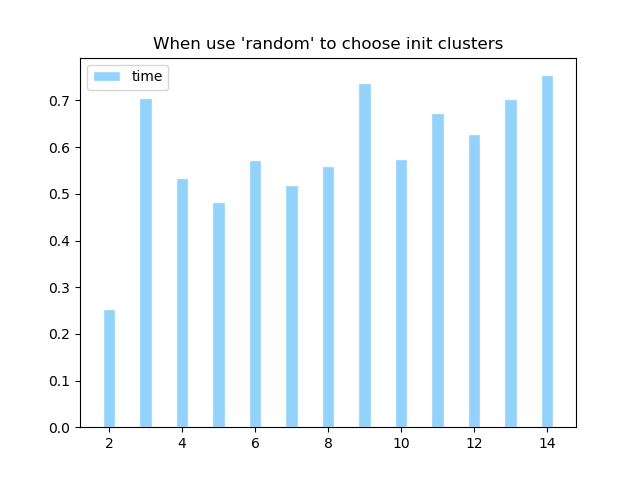
\includegraphics[width = 0.9\textwidth]{11.png}	
\end{center}
\end{figure}

\clearpage
\subsubsection{运行时间}
针对pluno、dptno、bndno字段,在2、4、8、16、32、64分别作为最小支持度时,运行时间:
\begin{figure}[!h]
\begin{center}
  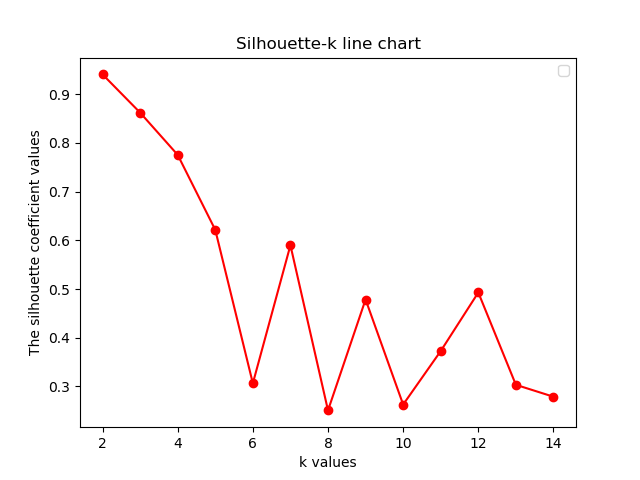
\includegraphics[width = 0.9\textwidth]{12.png}	
\end{center}
\end{figure}

\subsection{bii问针对三个字段的频繁集求取情况}
\subsubsection{频繁集个数}
针对pluno、dptno、bndno字段,在2、4、6、8、10分别作为最小支持度时,频繁集个数:


\begin{figure}[!h]
\begin{center}
  \includegraphics[width = 0.9\textwidth]{14.png}	
\end{center}
\end{figure}

\subsubsection{运行时间}
针对pluno、dptno、bndno字段,在2、4、6、8、10分别作为最小支持度时,运行时间:
\clearpage
\begin{figure}[!h]
\begin{center}
  \includegraphics[width = 0.9\textwidth]{13.png}	
\end{center}
\end{figure}

\section{分析讨论}
这里主要针对数据的预处理和ai、bi问的差异性来进行分析讨论。


\subsection{数据的预处理}
b问和a问的最大一点不同在于,b问需要考虑时序性,体现在本问当中的话,我是考虑将时间相同的数据合并作为一个值来考虑,也就是合并为$<a(ab)c>$的格式。

这里我的处理方法与a问的不同主要体现在最后一步合并上,大致的步骤如下:

1)仍然用字典来做存储,不过是两层字典。第一层的key为vipno值,value为一个字典;而第二层的这个字典,key为sldat,即时间,value为具体的item\_no值。

这样最终可以能够将时间相同的数据合并在了一起。


\subsection{a、b问的差异性}

首先说ai问和bi问。因为这两问都是针对uid去进行的数据合并,而对于同一个uid,其购买时间肯定是一样的,其合并后的结果和ai问是一样的,那么其实ai和bi的输入数据并没有太大的差异。我在这里选择出了支持度前十的针对pluno字段的频繁项集,其结果如下:

\begin{figure}[!h]
\begin{center}
  \includegraphics[width = 0.4\textwidth]{18.png}
  \caption{ai问}	
\end{center}
\end{figure}

\clearpage
\begin{figure}[!h]
\begin{center}
  \includegraphics[width = 0.4\textwidth]{15.png}	
  \caption{bi问(-1是分隔符)}
\end{center}
\end{figure}

显然,结果是一样的,这也符合我们的推测。

那么对于aii问和bii问,会不会有所不同呢?我同样是选择出了支持度前十的针对pluno字段的频繁项集,其结果如下:

\begin{figure}[!h]
\begin{center}
  \includegraphics[width = 0.4\textwidth]{16.png}
  \caption{ai问}	
\end{center}
\end{figure}

\begin{figure}[!h]
\begin{center}
  \includegraphics[width = 0.4\textwidth]{15.png}	
  \caption{bi问(-1是分隔符)}
\end{center}
\end{figure}

显然,结果出现了一定的差异,这是符合常理的,毕竟两种算法所运用到的原理存在着一定的差异性。与FP-growth算法不同的是,PrefixSpan算法引入了前缀、后缀的概念,即我们可以简单地理解为,出现在$a$后面的数据为$a$的后缀,而$a$就为这些数据的前缀。

那么就会出现这样一个情况,比如有$<a(bc)>$、$<(ab)>$这么两组数据,那么我们在计算$a$的后缀时,$b$要写作$b$、$_b$分别考虑,因为前者和$a$购买存在时间间隔,而后者则时间间隔在允许范围内,或者就是是同一次购买。这也是对应于FP-growth算法的一个很大的区别。

但是我发现支持度前十的频繁项集,还是存在着一定的相似度的,比如3038003、3038002都是排着前二的,而且其他频繁项集中对应的项也存在着一定的相似度。

那么我可以这样认为,对于本次作业的数据,虽然是否考虑时序性会对最终的频繁项集产生一定的影响,但是总体来说,本次作业的数据即超市购买信息和时间关系不大,也就是说,这些购买信息对应的用户的购买喜好并没有因为时间产生很大的差异性。当然至少对于本份数据是这样的。

\section{性能比较}

我们可以查看FP-growth和PrefixSpan算法两者的运行时间如下:

\begin{figure}[!h]
\begin{center}
  \includegraphics[width = 0.8\textwidth]{20.png}	
  \caption{FP-growth}
\end{center}
\end{figure}

\begin{figure}[!h]
\begin{center}
  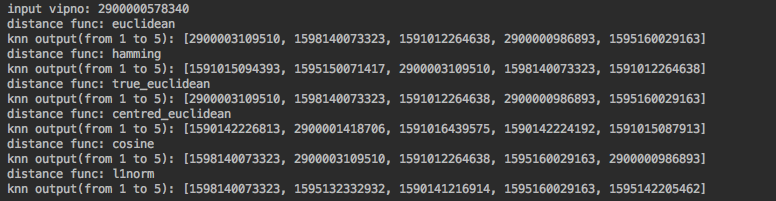
\includegraphics[width = 0.8\textwidth]{3.png}	
  \caption{PrefixSpan}
\end{center}
\end{figure}

总的来说差异不大,FP-growth会稍微快一点。考虑到本次数据大约有万级左右,并不算特别大,我可以粗略地认为这两种算法之间的性能相差不大。

\end{CJK}
\end{document}

